\documentclass{article}

%%% IDIOMA
\usepackage[spanish,english]{babel}
\addto\shorthandsspanish{\spanishdeactivate{~<>}}

%%% CODIFICACION Y FUENTES
\usepackage[utf8]{inputenc}
\usepackage[T1]{fontenc}
\usepackage{lmodern}
\usepackage{microtype}

%%% PAQUETES
\usepackage{amsmath}
\usepackage{graphicx}
\usepackage{booktabs}
\usepackage{array}
\usepackage{tabularx}
\usepackage{longtable}
\usepackage{multirow}
\usepackage{xcolor}
\usepackage{tcolorbox}
\usepackage{float}
\usepackage{pdflscape}
\usepackage{listings}
\usepackage[section]{placeins}
\usepackage[colorlinks=true,linkcolor=mxNavy,urlcolor=mxBlue,citecolor=mxNavy]{hyperref}

\definecolor{mxNavy}{HTML}{12405E}
\definecolor{mxBlue}{HTML}{2A85BE}
\definecolor{mxLight}{HTML}{EEF7FC}
\definecolor{mxGray}{HTML}{F5F7FA}

\newcolumntype{L}{>{\raggedright\arraybackslash}X}
\newcolumntype{R}{>{\raggedleft\arraybackslash}X}

\lstset{
  basicstyle=\ttfamily\footnotesize,
  backgroundcolor=\color{mxGray},
  frame=single,
  rulecolor=\color{mxBlue!40},
  breaklines=true,
  columns=fullflexible,
  keepspaces=true,
  showstringspaces=false,
  literate={á}{{\'a}}1 {é}{{\'e}}1 {í}{{\'i}}1 {ó}{{\'o}}1 {ú}{{\'u}}1 {ñ}{{\~n}}1 {Á}{{\'A}}1 {É}{{\'E}}1 {Í}{{\'I}}1 {Ó}{{\'O}}1 {Ú}{{\'U}}1 {Ñ}{{\~N}}1
}

%%% METADATOS DEL PROYECTO
\newcommand{\theCampus}{Campus Vitacura}
\newcommand{\theAssignment}{Sistemas de Información para la Gestión}
\newcommand{\theCourseCode}{ICN-292}
\newcommand{\theReportTitle}{Entrega 2 --- Solución SIG Final: Maxilux}
\newcommand{\theGroup}{Grupo 2}
\newcommand{\thePar}{100}
\newcommand{\theProfessor}{Patricio Eduardo Cifuentes Reyes}
\newcommand{\theAuthorA}{Juan Pablo Godoy Fajardo}
\newcommand{\theAuthorB}{Vicente Soto Martínez}
\newcommand{\theAuthorC}{Joaquín Tapia Mandiola}
\newcommand{\theAuthorD}{Claudio Vera Avila}
\newcommand{\theSemester}{Segundo Semestre 2026}

%%% MARGENES Y ENCABEZADOS
\usepackage[margin=22mm,inner=26mm]{geometry}
\usepackage{fancyhdr}
\setlength{\headheight}{42pt}
\setlength{\headsep}{10pt}

\pagestyle{fancy}
\fancyhf{}
\lhead{
\includegraphics[scale=0.28]{Logo usmUSM.png}}
\rhead{\small\color{gray} ICN-292 · Entrega 2 · Maxilux}
\renewcommand{\headrulewidth}{0.5pt}
\fancyfoot[C]{\textbf{\thepage}}

\makeatletter
\def\tableofcontents{%
 \newpage
 \centerline{\large\scshape Índice de contenidos}
 \vspace*{0.2in}
 \@mkboth{CONTENTS}{CONTENTS}
 \@starttoc{toc}
}
\makeatother

\hypersetup{pdftitle={ICN292 Entrega 2 - Maxilux}}

\begin{document}
\selectlanguage{spanish}
\hypersetup{pageanchor=false}

%------------------------------------------------------------------------------
% PORTADA
%------------------------------------------------------------------------------
\begin{titlepage}
\thispagestyle{empty}
\vspace*{0.8cm}
\begin{center}

\includegraphics[scale=0.48]{Logo usmUSM.png}
\end{center}
\vspace{1.5cm}
\begin{center}
\hrule
\vspace{3mm}
{\Huge \bfseries \theReportTitle}\\[0.45cm]
{\Large \theCourseCode\ --- \scshape \theAssignment}\\[0.25cm]
{\large Profesor: \theProfessor}
\vspace{4mm}
\hrule
\vspace{0.9cm}

\textbf{\theGroup} \quad -- \quad \textbf{Paralelo \thePar} \\[0.35cm]
\textbf{Integrantes:}\\[0.25cm]
\textbf{\theAuthorA} \\[0.18cm]
\textbf{\theAuthorB} \\[0.18cm]
\textbf{\theAuthorC} \\[0.18cm]
\textbf{\theAuthorD}

\vspace{0.6cm}
\textbf{Repositorio GitHub (Entrega 2):}\\[0.15cm]
{\small \url{https://github.com/JotaReyyyyyyyyyyyy/ICN292-E2-Maxilux} \quad (\texttt{tag: v1.1-e2})}

\vfill
\textsc{\theSemester}\\[0.35cm]
\textsc{\theCampus}
\end{center}
\end{titlepage}
\hypersetup{pageanchor=true}
\pagenumbering{arabic}

\tableofcontents
\clearpage

%==============================================================
\section{Resumen ejecutivo}
%==============================================================

\textbf{Problema de negocio.} \textbf{Maxilux} es una PYME comercializadora e intermediaria de iluminación industrial, comercial, vial y solar cuya operación recae en dos personas internas (Comercial/Operaciones y Finanzas/Proveedores), sin inventario propio masivo ni departamento de TI. El diagnóstico levantado desde la Entrega 1 evidenció tres cuellos de botella conectados: (1) la \textbf{prospección B2B} se realizaba manualmente sin memoria histórica (1,5\,h para armar una lista de 5 empresas y 5--6\,h en visitas en frío), junto con un gasto de \$400.000--\$600.000 mensuales en Google Ads donde 8 de cada 10 contactos resultaban no calificados; (2) la \textbf{documentación técnica} de sus 511 SKUs se confeccionaba manualmente en Canva, Word o PowerPoint (15--20 minutos por producto) o exponía directamente el PDF del proveedor (riesgo de desintermediación), mientras la planilla maestra de precios presentaba un 93,5\,\% de SKUs sin costo cargado y una fórmula contradictoria entre proveedor mínimo (\texttt{MINIFS}) y costo máximo (\texttt{MAX}); y (3) la \textbf{atención de consultas} carecía de repositorio centralizado, provocando tiempos de respuesta prolongados cada vez que faltaban especificaciones.

\textbf{Solución SIG implementada.} Se diseñó y materializó una solución integral auditable compuesta por:
\begin{itemize}
    \item \textbf{Base de datos relacional normalizada a 3FN} en SQLite~3 (\path{db/schema.sql} y \path{db/seed.sql}), con \textbf{16 tablas y 2 vistas calculadas} que unifican catálogo multi-proveedor, especificaciones técnicas sanitizadas, campañas/prospecciones con trazabilidad Ley~21.719 y registro de consultas/derivaciones, cargada con datos anonimizados coherentes con la escala real de la empresa y 0 violaciones de integridad referencial.
    \item \textbf{Automatización modular en n8n} (\path{automatizacion/}): cuatro flujos orquestados para prospección B2B (búsqueda IA con verificación literal de dominio, revisión humana en Google Sheets, creación idempotente de borradores IMAP sin envío automático, seguimiento tras 3 días hábiles y reporte PDF semanal por Telegram) más el flujo generador de fichas técnicas propias en XeLaTeX ($\le 2$ páginas) con filtro anti-marcas de proveedores.
    \item \textbf{Tablero KPI en localhost} con cobertura de catálogo, prospección y atención de consultas. Usa las siete consultas de \path{db/consultas.sql} y la base SQLite de demostración. Se inicia con \texttt{python -m app}.
\end{itemize}

\textbf{Resultados medibles verificados.} La solución consolidó los \textbf{511 SKUs} (14 grupos) en \textbf{133 fichas técnicas PDF} sin fuga alguna de marcas de proveedores, elevando la cobertura con respaldo técnico al \textbf{63,2\,\% (323 SKUs)} e identificando con exactitud que la brecha hacia la publicación final radica en dos atributos críticos (\textbf{Temperatura de operación} en 15,1\,\% y \textbf{Certificaciones} en 19,0\,\%, dejando 131 fichas en \texttt{BORRADOR} y 2 \texttt{APROBADA}). La vista de precios corrige la anomalía del Excel evitando un sobrecosto unitario acumulado de \textbf{\$197.000 CLP} sobre 32 SKUs multi-oferta sintéticos, la auditoría Ley~21.719 registra \textbf{0 infracciones} sobre empresas bloqueadas, y la simulación de consultas con ficha completa registra una resolución autónoma del \textbf{83,3\,\%} con un tiempo promedio de \textbf{25,3 minutos}.

\begin{table}[H]
\centering
\small
\begin{tabularx}{\textwidth}{lL}
\toprule
\textbf{Integrante} & \textbf{Responsabilidad E2} \\
\midrule
\theAuthorA & Evidencia, integración Sheets/n8n y gobernanza \\
\theAuthorB & Procesos BPMN, KPI y presentación \\
\theAuthorC & Modelo 3FN, arquitectura y automatización \\
\theAuthorD & Scripts SQL, consultas y reproducibilidad \\
\bottomrule
\end{tabularx}
\caption{Ficha del equipo ejecutor (Grupo 2, Paralelo 100).}
\end{table}

\clearpage

%==============================================================
\section{Trazabilidad E1 $\rightarrow$ E2 y contexto del caso}
%==============================================================

\subsection{Justificación de continuidad: Unter $\rightarrow$ Maxilux}

En la Entrega~1 (repositorio \url{https://github.com/Stump3412/ICN292-E1-Unter}) se modeló el caso de \emph{Unter}, distribuidora operada por dos personas. Al iniciar el despliegue técnico de la Entrega~2, los mismos dueños formalizaron la ejecución del sistema sobre \textbf{Maxilux}, empresa hermana perteneciente al mismo grupo controlador que opera bajo el mismo esquema de dos roles internos, idéntico modelo de compra contra pedido sin inventario masivo y los mismos tres problemas operativos. De hecho, en la transcripción de entrevista original de E1 ya figuraban menciones explícitas a iluminación y a campañas digitales que recibían consultas erróneas de distribuidoras eléctricas.

Conforme a la sección~2 del enunciado de Entrega~2, esta continuidad queda documentada y justificada en \path{docs/00-caso-pyme.md}, sujeta a ratificación formal del profesor de paralelo y respaldo documental del SII/acta. Trabajar sobre Maxilux permitió auditar activos reales completos: una lista maestra de \textbf{511 SKUs} en \textbf{14 grupos}, \textbf{55 fichas PDF de proveedores} y un catálogo web de \textbf{181 productos}.

\subsection{Matriz comparativa de evolución (qué se mantuvo, qué cambió y por qué)}

\begin{table}[H]
\centering
\small
\renewcommand{\arraystretch}{1.22}
\begin{tabularx}{\textwidth}{p{2.7cm}p{3.9cm}p{4.3cm}L}
\toprule
\textbf{Dimensión} & \textbf{Entrega 1 (Diagnóstico)} & \textbf{Entrega 2 (Solución final)} & \textbf{Por qué cambió} \\
\midrule
Identidad PYME & Unter (EPP y herramientas, 2 personas). & Maxilux (iluminación LED industrial, comercial, vial y solar; mismos dueños y 2 roles). & Disponibilidad de catálogo real completo (511 SKUs, 55 PDFs) y ejecución efectiva de n8n. \\
\addlinespace
Prospección B2B (BPMN + n8n) & 1 diagrama TO-BE lineal con puntaje numérico genérico. & 4 flujos n8n desacoplados + Worker Node + Sheets + IMAP + Telegram; sin puntajes opacos. & Garantizar idempotencia, tope de 100 pendientes, verificación literal de dominio y envío 100\,\% manual. \\
\addlinespace
Fichas técnicas & Proceso conceptual de armado asistido desde Word/PPT. & Generador consolidado Node/Python/XeLaTeX (511 SKUs $\rightarrow$ 133 PDFs $\le 2$ págs.) + disparo n8n. & El prototipo v1 por URL solo aceptaba 27/55 PDFs y creaba SKUs incompatibles con la lista real. \\
\addlinespace
Modelo de datos & ER preliminar de 9 entidades en diagrama conceptual. & Esquema SQLite~3 en \textbf{3FN estricta} con \textbf{16 tablas y 2 vistas} + \path{seed.sql} anonimizado. & Eliminar grupos repetitivos del Excel (77 cols) y JSON blobs del worker; corregir cálculo de costos. \\
\addlinespace
Módulo Atención / Chat IA & Modelado en BPMN TO-BE y RF-01..RF-11. & Modelado en BD 3FN (\texttt{consulta\_cliente}, \texttt{derivacion\_consulta}) y medido en Q7; chat en vivo como fase posterior. & Se priorizó resolver primero la base documental (fichas) de la cual depende RNF-01 antes de exponer un chat. \\
\bottomrule
\end{tabularx}
\caption{Trazabilidad estructural entre Entrega~1 y Entrega~2.}
\end{table}

%==============================================================
\section{Procesos BPMN finales y automatización en n8n}
%==============================================================

Los diagramas fuente AS-IS y TO-BE de la Entrega~1 permanecen en \path{assets/bpm/} y en el Anexo~\ref{anexo:bpmn_e1} para preservar el historial completo. Esta sección presenta los modelos TO-BE maduros de la Entrega~2 y su materialización exacta en flujos de \textbf{n8n}.

\subsection{Arquitectura lógica y física integrada}

La solución desacopla la orquestación visual (\textbf{n8n}) de la lógica transaccional y compilación (\textbf{Worker Node.js~24}, \textbf{Python~3} y \textbf{XeLaTeX/pdflatex}), evitando scripts frágiles dispersos y garantizando trazabilidad ante fallos. La Figura~\ref{fig:arq_sig} resume el flujo de datos entre fuentes externas, servicios locales y almacenamiento 3FN.

\begin{figure}[H]
\centering
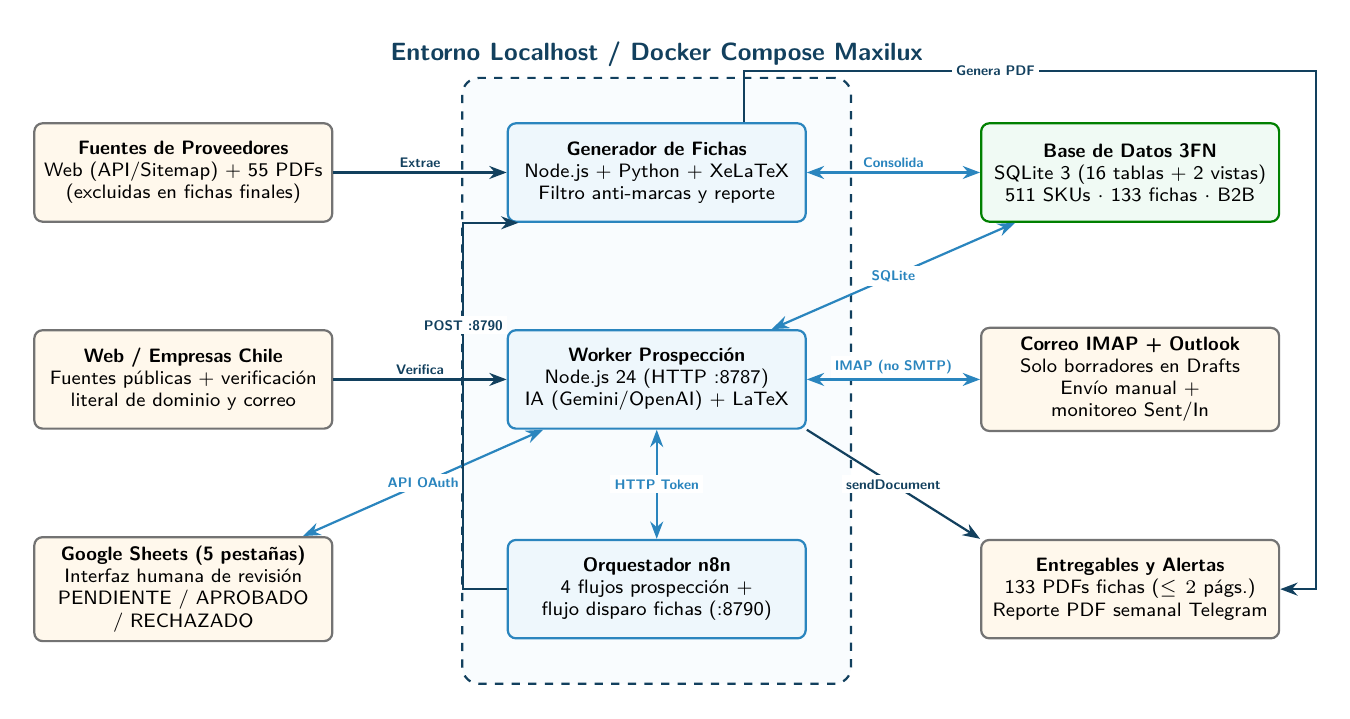
\includegraphics[width=\textwidth]{arquitectura_sig_maxilux.png}
\caption{Arquitectura integrada del SIG Maxilux en entorno localhost / Docker Compose.\label{fig:arq_sig}}
\end{figure}

\subsection{Proceso 1: Prospección B2B y seguimiento (4 flujos n8n)}

La prospección se descompuso en cuatro flujos exportados en \path{automatizacion/prospeccion/flujos/} (red Docker \url{http://worker:8787}) y \path{flujos-local/} (Windows localhost \url{http://127.0.0.1:8787}), todos autenticados mediante cabecera \texttt{x-maxilux-key} y protegidos por un bloqueo exclusivo en SQLite (\texttt{locks}) de 15 minutos.

\begin{table}[H]
\centering
\small
\renewcommand{\arraystretch}{1.2}
\begin{tabularx}{\textwidth}{p{2.6cm}p{2.0cm}p{4.6cm}L}
\toprule
\textbf{Flujo n8n} & \textbf{Disparador} & \textbf{Etapas HTTP / Nodos} & \textbf{Regla de negocio trazada al BPMN TO-BE} \\
\midrule
\texttt{01\_prospeccion} & Manual & \texttt{reviews} $\rightarrow$ \texttt{capacity} $\rightarrow$ \texttt{If (slots > 0)} $\rightarrow$ \texttt{discover} $\rightarrow$ \texttt{verify} $\rightarrow$ \texttt{compose} $\rightarrow$ \texttt{publish} & Sincroniza bloqueos previos; verifica cupo $< 100$ antes de llamar a la IA; busca máx. 10 empresas en 14 familias de catálogo; exige correo literal en HTML del mismo dominio y publica en \texttt{PENDIENTE}. \\
\addlinespace
\texttt{02\_borradores} & Manual & \texttt{reviews} $\rightarrow$ \texttt{approved} $\rightarrow$ \texttt{If (approved > 0)} $\rightarrow$ \texttt{draft} $\rightarrow$ \texttt{publish} & Procesa solo filas \texttt{APROBADO}; crea borrador IMAP en \texttt{Drafts} (\texttt{DELIVERY\_MODE=drafts} forzado, sin SMTP) con \texttt{Message-ID} determinista idempotente para recuperar ante caídas. \\
\addlinespace
\texttt{03\_seguimiento} & Manual + Cron \texttt{*/15 * * * *} & \texttt{reviews} $\rightarrow$ \texttt{mailbox} $\rightarrow$ \texttt{reconcile} $\rightarrow$ \texttt{due} $\rightarrow$ \texttt{If (due > 0)} $\rightarrow$ \texttt{queue} $\rightarrow$ \texttt{publish} & Escanea \texttt{Sent} e \texttt{INBOX} vía IMAP pasivo (\texttt{BODY.PEEK}); confirma envíos manuales desde Outlook; filtra respuestas \texttt{AUTO}; registra bajas/rebotes como bloqueo irreversible; tras \textbf{3 días hábiles} encola máx. 1 seguimiento \texttt{PENDIENTE}. \\
\addlinespace
\texttt{04\_resumen} & Manual + Cron \texttt{0 8 * * 0} & \texttt{reviews} $\rightarrow$ \texttt{period} $\rightarrow$ \texttt{If (!alreadySent)} $\rightarrow$ \texttt{summarize} $\rightarrow$ \texttt{render} $\rightarrow$ \texttt{deliver} $\rightarrow$ \texttt{publish} & \textbf{Sin llamadas a IA.} Consolida movimientos semanales desde SQLite, compila PDF LaTeX con portada y lo entrega vía Telegram (\texttt{sendDocument}) con bandera \texttt{uncertain} anti-duplicados. \\
\bottomrule
\end{tabularx}
\caption{Trazabilidad entre flujos n8n y reglas del BPMN TO-BE de prospección.}
\end{table}

\textbf{Auditoría y mejoras aplicadas al paquete de prospección.} Durante la revisión técnica de \path{Maxilux_para_JuanPablo.zip} se detectaron y corrigieron cinco brechas críticas en la copia operativa recreada sobre la cuenta Google Sheets del equipo: (a) ampliación de los prompts y la \emph{skill} comercial desde 6 líneas parciales hacia las \textbf{14 familias reales del catálogo} (incluyendo Solar y Batería con 22,7\,\% de SKUs, Alumbrado Público y Postes); (b) ajuste del modelo nativo \texttt{openai}/\texttt{gpt-6-luna} a \texttt{reasoning.effort=medium} (manteniendo Gemini como alternativa opcional) y aumento del tope mensual desde \texttt{USD 0.50} a \texttt{LLM\_BUDGET\_USD=5.00} para cubrir múltiples lotes sin bloqueo prematuro; (c) parametrización opcional de la firma web (\texttt{MAIL\_WEBSITE}) mientras no se confirme la web pública; (d) limpieza de una referencia residual externa en \texttt{SKILL.md}; y (e) generación de \texttt{flujos-local/} y lanzador Windows sin Docker, manteniendo los \textbf{66 tests unitarios} y validaciones de seguridad (\texttt{npm run check}) aprobados al 100\,\%.

\subsection{Proceso 2: Generación consolidada de fichas técnicas}

El proceso de fichas técnicas evolucionó desde un primer prototipo n8n de 34 nodos por URL (\path{Maxilux_Fichas_n8n.json}) hacia un generador consolidado (\path{Maxilux_Generar_Fichas.json} + servicio HTTP local en puerto \texttt{8790}). El prototipo inicial se descartó como flujo principal porque solo aceptaba 27 de los 55 PDFs reales y generaba códigos correlativos (\texttt{MX-CAM-0001}) incompatibles con la lista de precios real (\texttt{MX-1000..MX-1510}). La versión productiva fusiona la lista maestra, el catálogo extraído de PDFs y datos web estructurados de proveedores, corrige erratas automáticas, separa fichas por IP distinto, aplica una expresión regular anti-marcas que aborta la compilación ante cualquier nombre de proveedor, y genera \textbf{133 PDFs en XeLaTeX} ($\le 2$ páginas) más un reporte estructurado de brechas (\texttt{reporte.xlsx}).

\begin{landscape}
\thispagestyle{plain}
\begin{figure}[H]
\centering
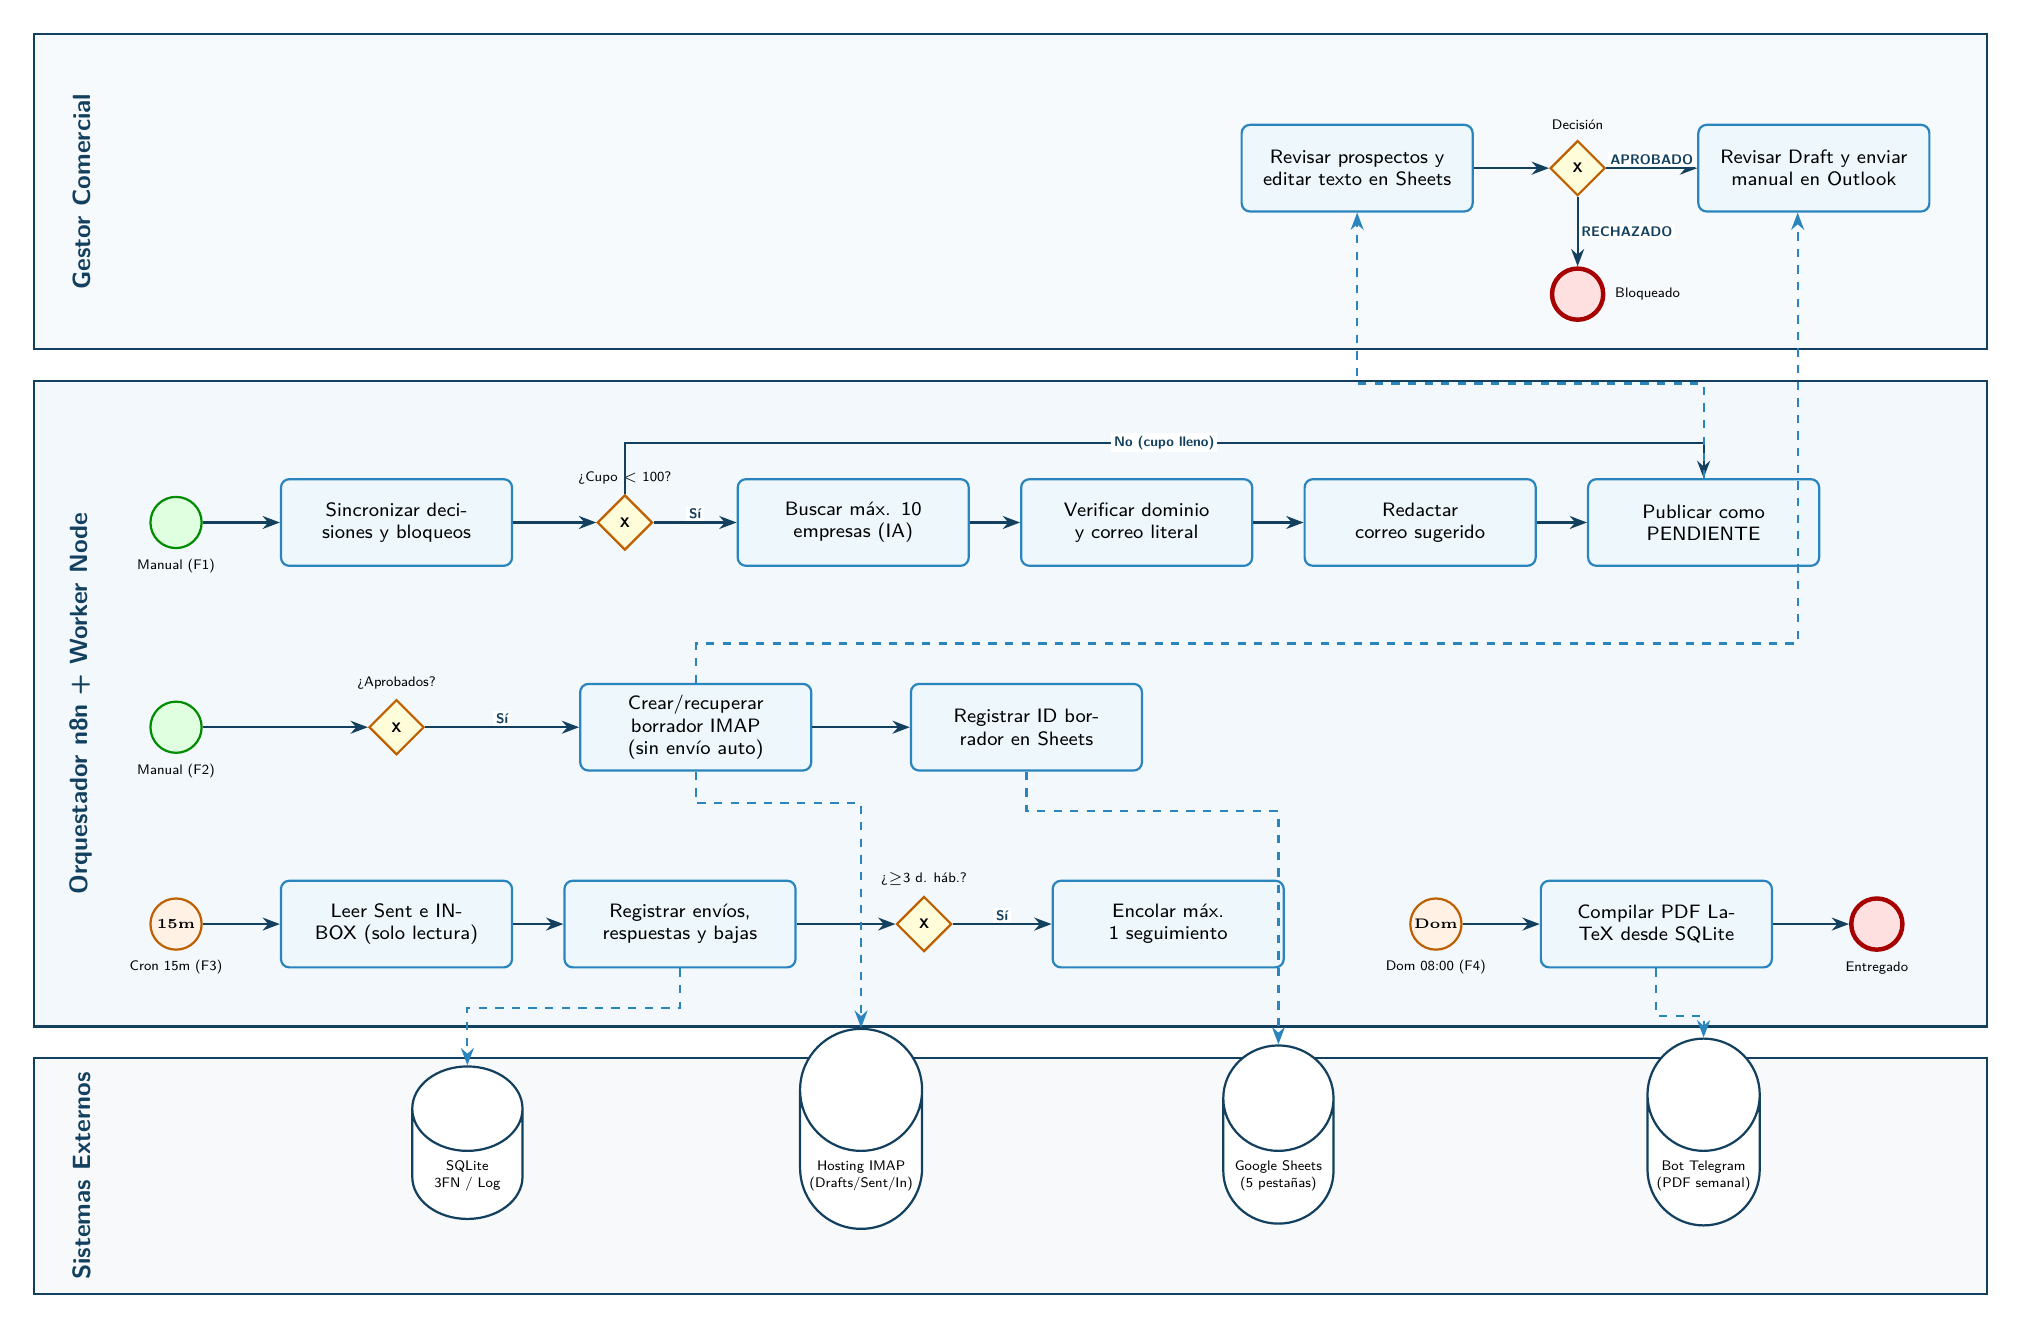
\includegraphics[width=\linewidth,height=0.84\textheight,keepaspectratio]{bpmn_prospeccion_tobe_e2.png}
\caption{Diagrama BPMN TO-BE final (Entrega~2) del proceso de prospección B2B trazado a los cuatro flujos n8n.\label{fig:bpmn_pros_e2}}
\end{figure}
\end{landscape}

\begin{landscape}
\thispagestyle{plain}
\begin{figure}[H]
\centering
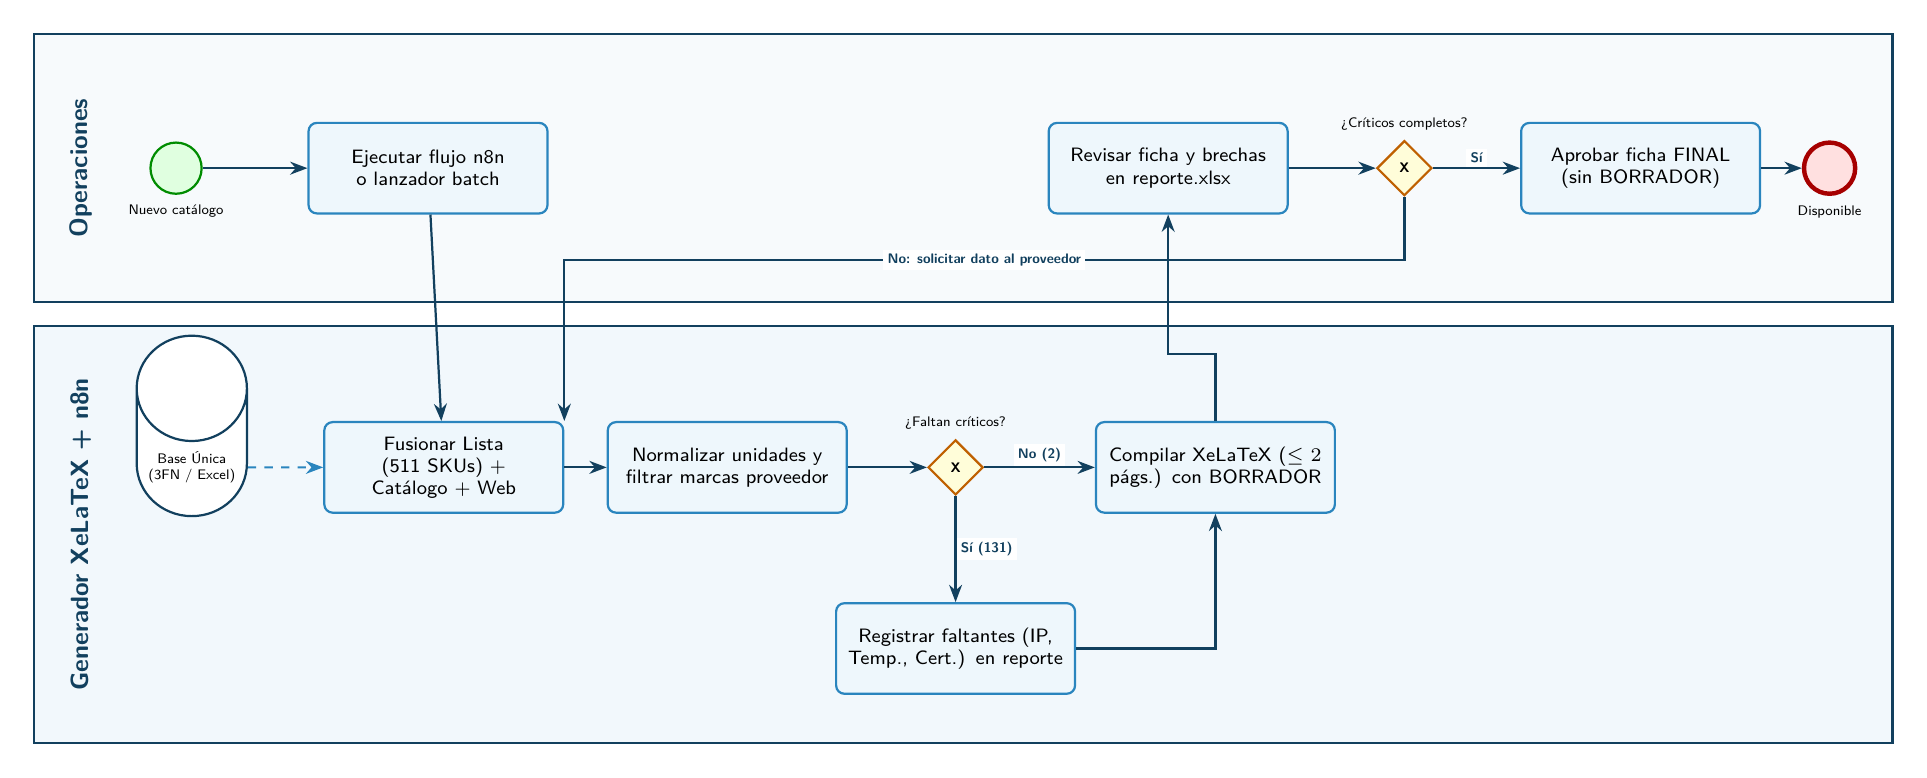
\includegraphics[width=\linewidth,height=0.84\textheight,keepaspectratio]{bpmn_fichas_tobe_e2.png}
\caption{Diagrama BPMN TO-BE final (Entrega~2) de generación consolidada de fichas técnicas.\label{fig:bpmn_fich_e2}}
\end{figure}
\end{landscape}

%==============================================================
\section{Modelo de datos ER en 3FN y diccionario de datos}
%==============================================================

\subsection{Anomalías en las fuentes originales y demostración 1FN $\rightarrow$ 2FN $\rightarrow$ 3FN}

La auditoría técnica de las herramientas previas reveló que ninguna almacenaba datos en Tercera Forma Normal:
\begin{itemize}
    \item \textbf{Lista de precios Excel (\texttt{LISTA DE PRECIOS OCTUBRE 2026.xlsx}):} 10 hojas donde solo 33 de 511 SKUs (6,5\,\%) tienen costo cargado, falta una pestaña propia para uno de los tres proveedores principales, y la columna \texttt{ORIGEN} calcula el menor costo (\texttt{MINIFS}) mientras \texttt{COSTO} toma el máximo (\texttt{=MAX(M:T)}), generando un error latente al comparar dos proveedores.
    \item \textbf{Base plana de fichas (\texttt{Base de fichas Maxilux.xlsx}):} 511 filas $\times$ 77 columnas con grupos repetitivos (\texttt{Característica 1..6}) y dependencias transitivas de grupo, serie, ficha y proveedor.
    \item \textbf{SQLite operativo del worker (\texttt{src/core.mjs}):} tabla \texttt{leads(id, payload)} con todo el objeto serializado en JSON (violación de 1FN).
\end{itemize}

\begin{table}[H]
\centering
\small
\renewcommand{\arraystretch}{1.2}
\begin{tabularx}{\textwidth}{p{2.2cm}p{4.3cm}p{4.7cm}L}
\toprule
\textbf{Nivel} & \textbf{Incumplimiento previo} & \textbf{Corrección en \texttt{schema.sql}} & \textbf{Anomalía evitada} \\
\midrule
\textbf{1FN} & Columnas enumeradas (\texttt{Característica 1..6}) y objetos JSON en \texttt{leads.payload}. & Cero JSON blobs y cero grupos repetitivos. Cada dato técnico vive en \texttt{especificacion\_producto (sku, id\_atributo)} y cada correo IMAP en \texttt{interaccion\_prospeccion}. & Imposibilidad de consultar o indexar atributos individuales mediante SQL estándar. \\
\addlinespace
\textbf{2FN} & En una tabla combinada producto--proveedor, nombre o potencia dependen solo de \texttt{sku}, no de \texttt{(sku, id\_proveedor)}. & Separación de \texttt{producto (sku PK)} y \texttt{oferta\_proveedor (UNIQUE(sku, id\_proveedor))} más \texttt{especificacion\_producto}. & Anomalía de actualización o incapacidad de registrar un SKU sin oferta vigente. \\
\addlinespace
\textbf{3FN} & \texttt{ficha\_tecnica} mezclaba grupo y conteos derivados; \texttt{producto} mezclaba precios calculados y proveedor; \texttt{prospeccion} mezclaba empresa, contacto y campaña. & Extracción de \texttt{grupo\_producto}, \texttt{serie\_comercial}, \texttt{proveedor}, \texttt{empresa\_cliente}, \texttt{contacto} y \texttt{campana\_prospeccion}. Conteos críticos y precios (\(\times 1{,}65\), \(\times 1{,}52\), \(\times 1{,}42\)) se calculan en vistas. & Anomalía de borrado (perder historial de empresa al cerrar campaña) y precios desincronizados. \\
\bottomrule
\end{tabularx}
\caption{Demostración formal de normalización a Tercera Forma Normal (3FN).}
\end{table}

\begin{landscape}
\thispagestyle{plain}
\begin{figure}[H]
\centering
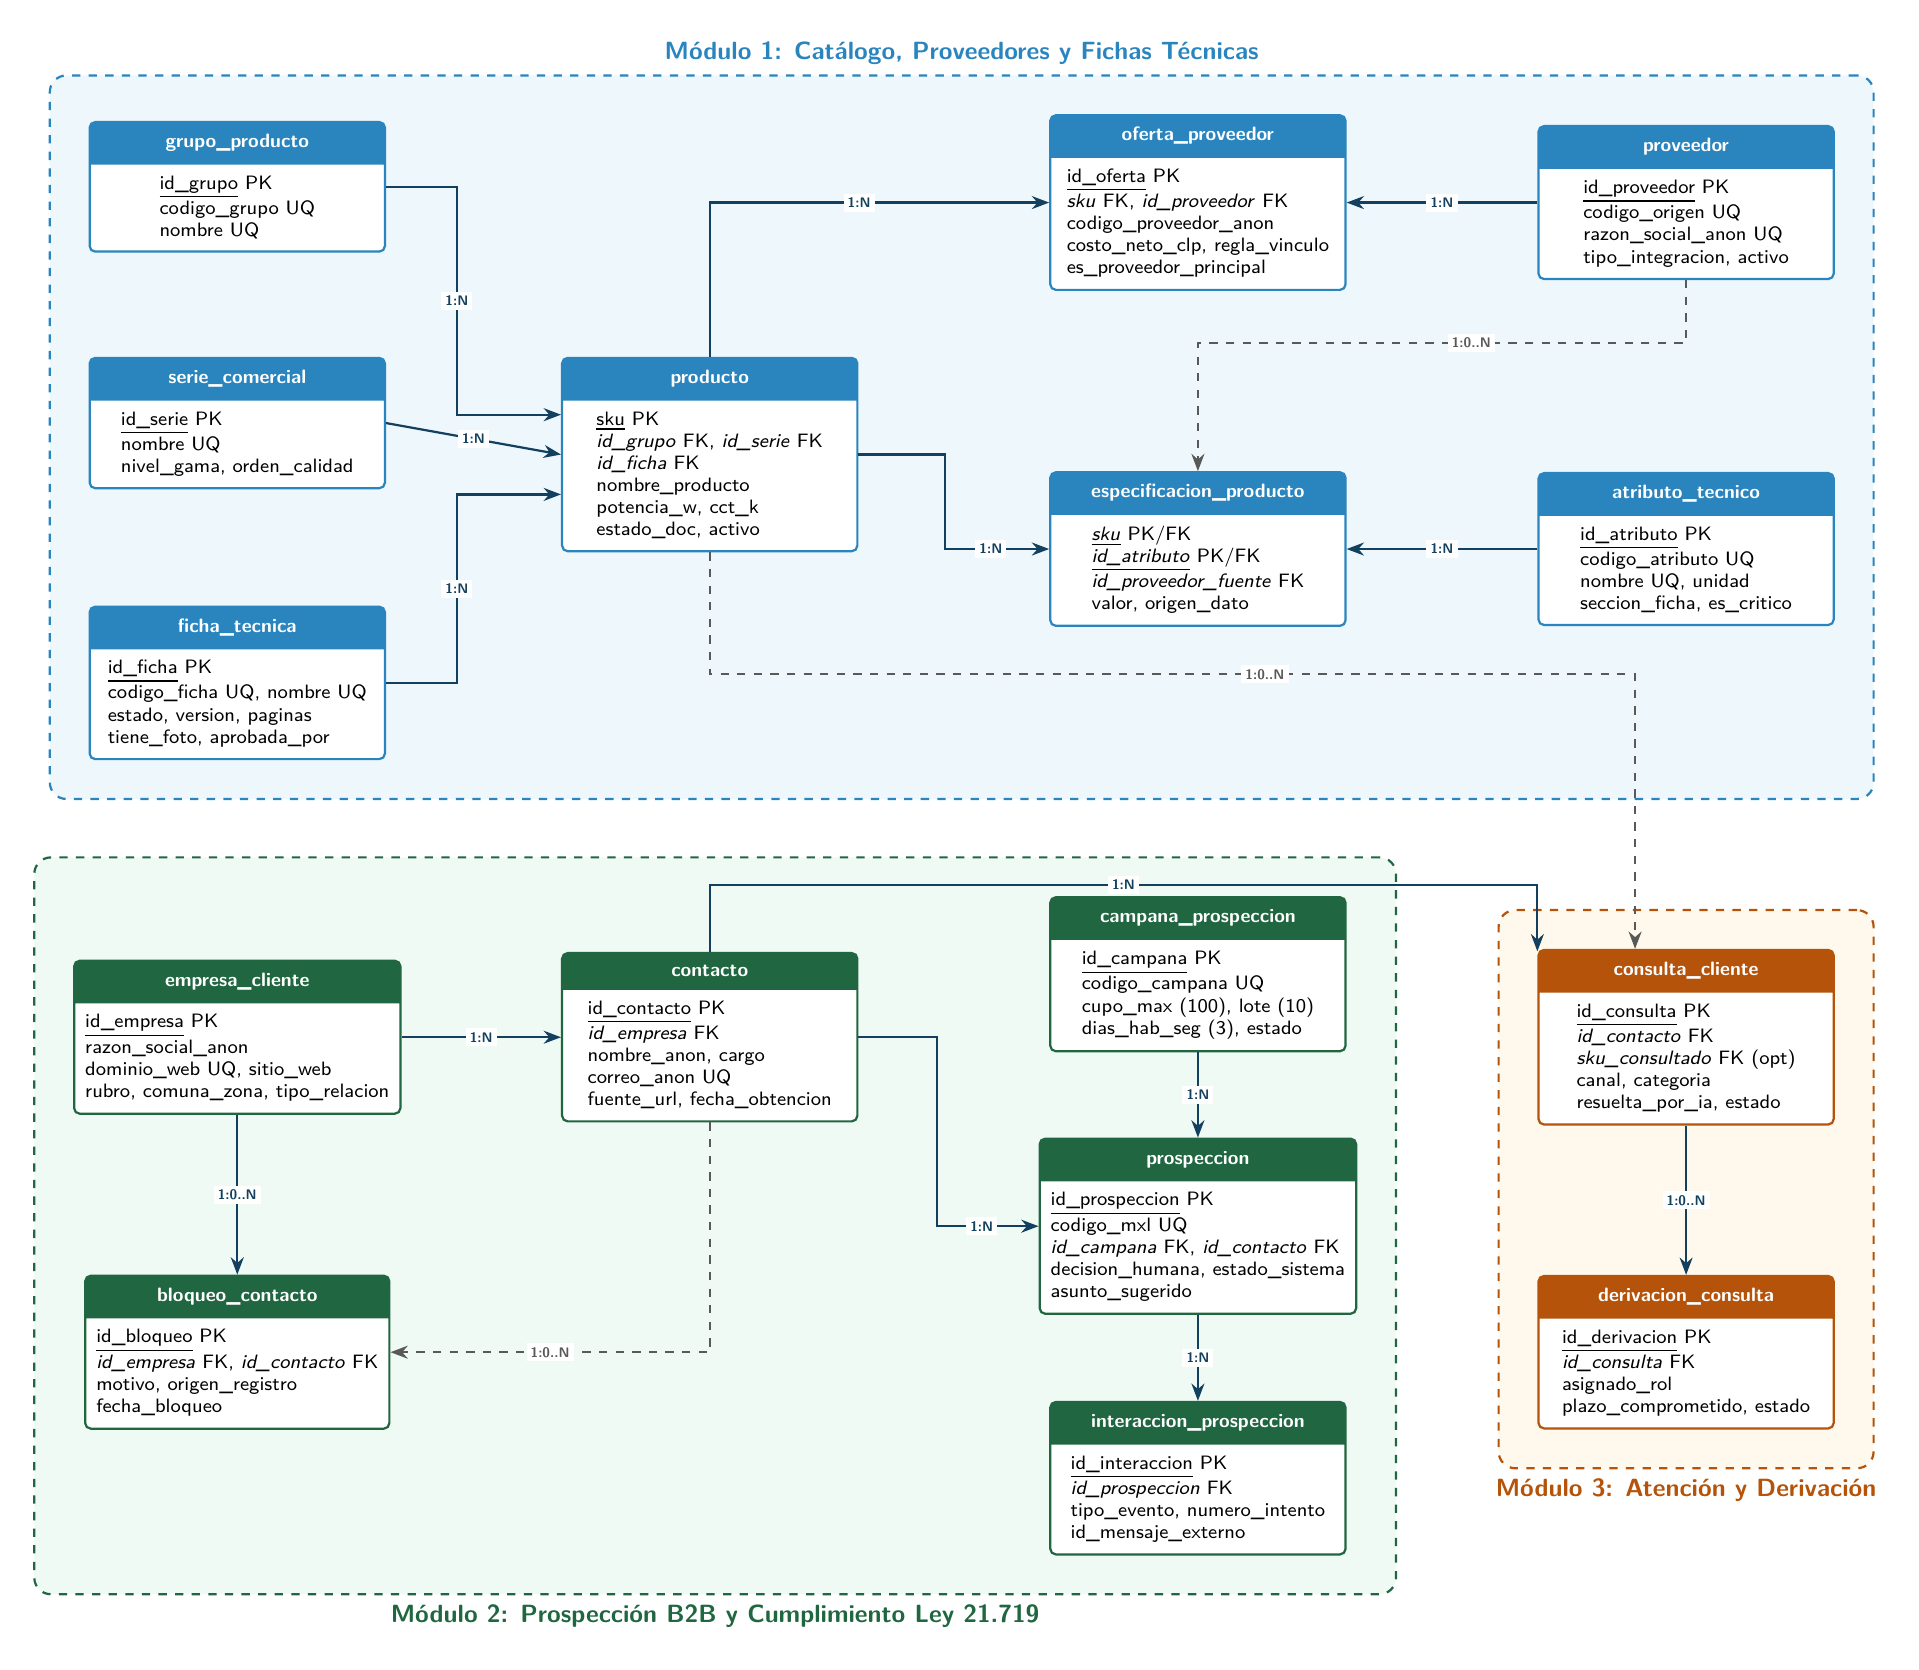
\includegraphics[width=\linewidth,height=0.86\textheight,keepaspectratio]{er_maxilux_3fn.png}
\caption{Diagrama Entidad--Relación normalizado a 3FN del SIG Maxilux (16 tablas en 3 módulos).\label{fig:er_3fn}}
\end{figure}
\end{landscape}

\subsection{Diccionario de datos (16 tablas y 2 vistas)}

Todas las tablas incorporan llaves primarias explícitas (\texttt{PK}), llaves foráneas con integridad referencial (\texttt{PRAGMA foreign\_keys = ON}), restricciones \texttt{UNIQUE} y validaciones de dominio \texttt{CHECK}.

\begin{longtable}{p{3.4cm}p{2.9cm}p{4.1cm}p{4.6cm}}
\toprule
\textbf{Tabla} & \textbf{PK / UQ} & \textbf{Claves foráneas (FK)} & \textbf{Atributos clave y reglas de negocio} \\
\midrule
\endfirsthead
\toprule
\textbf{Tabla} & \textbf{PK / UQ} & \textbf{Claves foráneas (FK)} & \textbf{Atributos clave y reglas de negocio} \\
\midrule
\endhead
\texttt{grupo\_producto} & \texttt{id\_grupo} (PK), \texttt{codigo\_grupo} (UQ) & --- & \texttt{nombre} (UQ, 14 categorías), \texttt{descripcion}. \\
\texttt{serie\_comercial} & \texttt{id\_serie} (PK), \texttt{nombre} (UQ) & --- & \texttt{nivel\_gama} (\texttt{BASICA}.. \texttt{PROFESIONAL}), \texttt{orden\_calidad}. \\
\texttt{proveedor} & \texttt{id\_proveedor} (PK), \texttt{codigo\_origen} (UQ) & --- & \texttt{razon\_social\_anon} (UQ), \texttt{tipo\_integracion}, \texttt{activo}. \\
\texttt{ficha\_tecnica} & \texttt{id\_ficha} (PK), \texttt{codigo\_ficha} (UQ) & --- & \texttt{estado} (\texttt{BORRADOR}/\texttt{APROBADA}), \texttt{paginas} (1--2), \texttt{CHECK} exige aprobador y fecha si está \texttt{APROBADA}. \\
\texttt{producto} & \texttt{sku} (PK) & \texttt{id\_grupo}, \texttt{id\_serie}, \texttt{id\_ficha} & \texttt{nombre\_producto}, \texttt{potencia\_w} ($>0$), \texttt{cct\_k}, \texttt{estado\_doc} (\texttt{COMPLETA}/\texttt{BORRADOR}/\texttt{SIN\_RESPALDO}). \\
\texttt{oferta\_proveedor} & \texttt{id\_oferta} (PK), \texttt{UQ(sku, id\_prov)} & \texttt{sku}, \texttt{id\_proveedor} & \texttt{codigo\_proveedor\_anon}, \texttt{costo\_neto\_clp} ($>0$), \texttt{regla\_vinculo}, \texttt{es\_proveedor\_principal}. \\
\texttt{atributo\_tecnico} & \texttt{id\_atributo} (PK), \texttt{codigo\_atributo} (UQ) & --- & \texttt{nombre}, \texttt{unidad}, \texttt{seccion\_ficha}, \texttt{es\_critico} (1 para IP, Temp., Cert.). \\
\texttt{especificacion\_producto} & \texttt{PK(sku, id\_atributo)} & \texttt{sku}, \texttt{id\_atributo}, \texttt{id\_proveedor\_fuente} & \texttt{valor} (filtrado contra marcas), \texttt{origen\_dato}, \texttt{fecha\_captura}. \\
\texttt{empresa\_cliente} & \texttt{id\_empresa} (PK), \texttt{dominio\_web} (UQ) & --- & \texttt{razon\_social\_anon}, \texttt{rubro}, \texttt{sitio\_web}, \texttt{comuna\_zona}, \texttt{tipo\_relacion}. \\
\texttt{contacto} & \texttt{id\_contacto} (PK), \texttt{correo\_anon} (UQ) & \texttt{id\_empresa} & \texttt{nombre\_anon}, \texttt{cargo}, \texttt{fuente\_url}, \texttt{fecha\_obtencion}, \texttt{verificado\_dominio}. \\
\texttt{campana\_prospeccion} & \texttt{id\_campana} (PK), \texttt{codigo\_campana} (UQ) & --- & \texttt{cupo\_max\_pendientes} (100), \texttt{lote\_por\_corrida} (10), \texttt{dias\_habiles\_seguimiento} (3). \\
\texttt{prospeccion} & \texttt{id\_prospeccion} (PK), \texttt{codigo\_mxl} (UQ) & \texttt{id\_campana}, \texttt{id\_contacto} & \texttt{decision\_humana} (\texttt{PENDIENTE}/\texttt{APROBADO}/\texttt{RECHAZADO}), \texttt{estado\_sistema}, \texttt{asunto\_sugerido}. \\
\texttt{interaccion\_prospeccion} & \texttt{id\_interaccion} (PK) & \texttt{id\_prospeccion} & \texttt{tipo\_evento} (Draft, Envío, Respuesta, Auto, Rebote, Baja), \texttt{id\_mensaje\_externo}, \texttt{fecha\_evento}. \\
\texttt{bloqueo\_contacto} & \texttt{id\_bloqueo} (PK) & \texttt{id\_empresa}, \texttt{id\_contacto} (opt) & \texttt{motivo} (\texttt{RECHAZADO\_EN\_PLANILLA}, \texttt{BAJA\_TITULAR}, \texttt{REBOTE\_CORREO}), \texttt{origen\_registro}. \\
\texttt{consulta\_cliente} & \texttt{id\_consulta} (PK) & \texttt{id\_contacto}, \texttt{sku\_consultado} (opt) & \texttt{canal}, \texttt{categoria}, \texttt{resuelta\_por\_ia}, \texttt{estado}, \texttt{fecha\_ingreso}, \texttt{fecha\_respuesta}. \\
\texttt{derivacion\_consulta} & \texttt{id\_derivacion} (PK) & \texttt{id\_consulta} & \texttt{asignado\_rol} (\texttt{COMERCIAL\_OPERACIONES} / \texttt{FINANZAS\_PROVEEDORES}), \texttt{plazo\_comprometido}, \texttt{estado}. \\
\bottomrule
\caption{Diccionario resumido de las 16 tablas normalizadas en \texttt{db/schema.sql}.}
\end{longtable}

Además, se definen dos vistas calculadas en \texttt{db/schema.sql} para garantizar la ausencia total de redundancia y atributos derivados almacenados:

\begin{lstlisting}[language=SQL,caption={Vistas calculadas en db/schema.sql (precios mínimos y cobertura crítica).}]
CREATE VIEW v_lista_precios_clientes AS
SELECT p.sku, g.nombre AS grupo, p.nombre_producto, p.cct_k,
       COUNT(o.id_oferta) AS cantidad_ofertas,
       MIN(o.costo_neto_clp) AS costo_minimo_clp,
       MAX(o.costo_neto_clp) AS costo_maximo_clp,
       ROUND(MIN(o.costo_neto_clp) * 1.65, 0) AS precio_proyecto_clp,
       ROUND(MIN(o.costo_neto_clp) * 1.52, 0) AS precio_descuento_clp,
       ROUND(MIN(o.costo_neto_clp) * 1.42, 0) AS precio_final_clp
FROM producto p
JOIN grupo_producto g ON g.id_grupo = p.id_grupo
JOIN oferta_proveedor o ON o.sku = p.sku
GROUP BY p.sku, g.nombre, p.nombre_producto, p.cct_k;
\end{lstlisting}

La vista \texttt{v\_cobertura\_fichas} complementa este diseño calculando por cada ficha técnica el total de modelos asociados, los modelos con respaldo técnico y la cantidad de SKUs sin \texttt{IP}, \texttt{TEMP\_OPERACION} o \texttt{CERTIFICACIONES}.

%==============================================================
\section{Diseño SQL, datos anonimizados y consultas de negocio}
%==============================================================

\subsection{Criterio de motor y política de anonimización}

Se eligió \textbf{SQLite~3} como motor SQL entregable por ser transaccional, soportar restricciones \texttt{FOREIGN KEY} y \texttt{CHECK} completas, coincidir nativamente con la persistencia del worker Node.js y garantizar portabilidad inmediata en cualquier computador limpio (incluido de serie en Python~3 sin instalación ni credenciales de servidor).

El script \path{db/seed.sql} (3.080 líneas) respeta íntegramente la privacidad y confidencialidad de la PYME:
\begin{itemize}
    \item \textbf{Catálogo y especificaciones (escala real anonimizada):} 14 grupos, 5 series, 8 proveedores genéricos (\texttt{P01}--\texttt{P08}), \textbf{511 productos} (\texttt{MX-1000} a \texttt{MX-1510}), \textbf{133 fichas técnicas} (2 \texttt{APROBADA}, 131 \texttt{BORRADOR}) y \textbf{1.827 especificaciones técnicas} filtradas contra cualquier mención de marca o URL de proveedor.
    \item \textbf{Ofertas económicas sintéticas:} 370 filas en \texttt{oferta\_proveedor} con costos unitarios sintéticos coherentes por categoría y potencia (incluyendo 32 SKUs con ofertas competidoras de 2--3 proveedores), sin exponer ningún costo real del Excel de la empresa.
    \item \textbf{Prospección y atención sintéticas:} 25 empresas bajo dominios reservados \texttt{.example} (RFC~2606), 30 contactos, 3 campañas, 25 prospecciones, 35 interacciones IMAP, 5 bloqueos Ley~21.719, 24 consultas de clientes y 15 derivaciones internas.
\end{itemize}

\subsection{Resultados ejecutados e interpretación (Q1 a Q7)}

Al ejecutar \texttt{python db/ejecutar.py}, \texttt{PRAGMA foreign\_key\_check} retorna \textbf{0 violaciones} y las 7 consultas de \path{db/consultas.sql} entregan los resultados exactos que se reportan e interpretan a continuación.

\subsubsection*{Q1: Cobertura técnica y estado de fichas por grupo de producto}

\begin{lstlisting}[language=SQL,caption={Consulta Q1 en db/consultas.sql.}]
SELECT g.nombre AS grupo, COUNT(DISTINCT p.sku) AS total_skus,
       COUNT(DISTINCT f.id_ficha) AS fichas_totales,
       COUNT(DISTINCT CASE WHEN f.estado = 'APROBADA' THEN f.id_ficha END) AS fichas_aprobadas,
       COUNT(DISTINCT CASE WHEN f.estado = 'BORRADOR' THEN f.id_ficha END) AS fichas_borrador,
       SUM(CASE WHEN p.estado_doc <> 'SIN_RESPALDO' THEN 1 ELSE 0 END) AS skus_con_datos,
       SUM(CASE WHEN p.estado_doc = 'SIN_RESPALDO' THEN 1 ELSE 0 END) AS skus_sin_respaldo,
       ROUND(100.0 * SUM(CASE WHEN p.estado_doc <> 'SIN_RESPALDO' THEN 1 ELSE 0 END) / COUNT(*), 1) AS pct_con_datos
FROM producto p
JOIN grupo_producto g ON g.id_grupo = p.id_grupo
JOIN ficha_tecnica f ON f.id_ficha = p.id_ficha
GROUP BY g.id_grupo, g.nombre ORDER BY total_skus DESC, g.nombre ASC;
\end{lstlisting}

\begin{table}[H]
\centering
\scriptsize
\begin{tabularx}{\textwidth}{Lrrrrrrr}
\toprule
\textbf{Grupo} & \textbf{SKUs} & \textbf{Fichas} & \textbf{Aprob.} & \textbf{Borr.} & \textbf{Con datos} & \textbf{Sin resp.} & \textbf{\% Respaldo} \\
\midrule
PANEL LED & 120 & 22 & 0 & 22 & 114 & 6 & 95,0\,\% \\
SOLAR Y BATERÍA & 116 & 18 & 2 & 16 & 42 & 74 & 36,2\,\% \\
PROYECTOR & 63 & 7 & 0 & 7 & 57 & 6 & 90,5\,\% \\
LUMINARIA CALLE & 38 & 4 & 0 & 4 & 13 & 25 & 34,2\,\% \\
CAMPANA & 33 & 5 & 0 & 5 & 20 & 13 & 60,6\,\% \\
POSTE & 26 & 25 & 0 & 25 & 3 & 23 & 11,5\,\% \\
ANTIEXPLOSIVO & 25 & 6 & 0 & 6 & 15 & 10 & 60,0\,\% \\
TUBO LED & 24 & 12 & 0 & 12 & 24 & 0 & 100,0\,\% \\
AMPOLLETA & 20 & 7 & 0 & 7 & 10 & 10 & 50,0\,\% \\
EMERGENCIA & 17 & 13 & 0 & 13 & 14 & 3 & 82,4\,\% \\
CANOA & 12 & 8 & 0 & 8 & 10 & 2 & 83,3\,\% \\
FAROL PLAZA & 9 & 1 & 0 & 1 & 0 & 9 & 0,0\,\% \\
APLIQUE & 4 & 4 & 0 & 4 & 1 & 3 & 25,0\,\% \\
FOCO & 4 & 1 & 0 & 1 & 0 & 4 & 0,0\,\% \\
\midrule
\textbf{Total catálogo} & \textbf{511} & \textbf{133} & \textbf{2} & \textbf{131} & \textbf{323} & \textbf{188} & \textbf{63,2\,\%} \\
\bottomrule
\end{tabularx}
\caption{Resultado real ejecutado de Q1: cobertura documental por grupo de producto.}
\end{table}

\textbf{Interpretación de negocio:} El generador automático logra respaldar con especificaciones técnicas al \textbf{63,2\,\% del catálogo (323 SKUs)} consolidados en 133 fichas sin marcas de terceros. Mientras \texttt{TUBO LED} (100\,\%), \texttt{PANEL LED} (95,0\,\%) y \texttt{PROYECTOR} (90,5\,\%) tienen cobertura casi total, \texttt{SOLAR Y BATERÍA} (segundo grupo del catálogo con 116 SKUs, solo 36,2\,\% respaldado), \texttt{LUMINARIA CALLE} (34,2\,\%) y \texttt{POSTE} (11,5\,\%) concentran la mayor brecha técnica debido a accesorios y equipos que los proveedores no publican en línea.

\subsubsection*{Q2: Ranking de atributos críticos que bloquean la aprobación}

\begin{table}[H]
\centering
\scriptsize
\begin{tabularx}{\textwidth}{lLrrrrr}
\toprule
\textbf{Código} & \textbf{Atributo crítico} & \textbf{SKUs c/dato} & \textbf{Faltantes total} & \textbf{Con ficha s/dato} & \textbf{Fichas bloq.} & \textbf{\% Cobertura} \\
\midrule
\texttt{TEMP\_OPERACION} & Temperatura de operación & 77 & 434 & 246 & 128 & 15,1\,\% \\
\texttt{CERTIFICACIONES} & Certificaciones & 97 & 414 & 226 & 124 & 19,0\,\% \\
\texttt{IP} & Grado de protección IP & 278 & 233 & 45 & 85 & 54,4\,\% \\
\bottomrule
\end{tabularx}
\caption{Resultado real ejecutado de Q2: atributos críticos faltantes.}
\end{table}

\textbf{Interpretación de negocio:} De las 133 fichas generadas, 131 salen con marca de agua \texttt{BORRADOR} principalmente porque los proveedores omiten \textbf{Temperatura de operación} (cubre solo 15,1\,\%, bloquea 128 fichas) y \textbf{Certificaciones} (19,0\,\%, bloquea 124 fichas), incluso en 246 y 226 SKUs que ya cuentan con ficha técnica vinculada. Esto entrega a Finanzas/Proveedores una lista priorizada exacta de qué datos exigir a cada fabricante.

\subsubsection*{Q3: Comparativo multi-proveedor y corrección del cálculo de costos (\texttt{MIN} vs \texttt{MAX})}

\begin{table}[H]
\centering
\scriptsize
\begin{tabularx}{\textwidth}{Lrrrrrr}
\toprule
\textbf{Grupo} & \textbf{\shortstack{SKU\\multioferta}} & \textbf{\shortstack{Costo mín.\\prom.}} & \textbf{\shortstack{Costo máx.\\prom.}} & \textbf{\shortstack{Diferencia\\acumulada}} & \textbf{\shortstack{Proyecto\\($\times 1{,}65$)}} & \textbf{\shortstack{Final\\($\times 1{,}42$)}} \\
\midrule
SOLAR Y BATERÍA & 4 & \$73.525 & \$89.150 & \$62.500 & \$121.316 & \$104.406 \\
PROYECTOR & 8 & \$51.800 & \$59.063 & \$58.100 & \$85.470 & \$73.556 \\
CAMPANA & 3 & \$69.633 & \$84.433 & \$44.400 & \$114.895 & \$98.879 \\
PANEL LED & 17 & \$10.818 & \$12.700 & \$32.000 & \$17.849 & \$15.361 \\
\bottomrule
\end{tabularx}
\caption{Resultado real ejecutado de Q3 sobre la vista \texttt{v\_lista\_precios\_clientes} (valores sintéticos CLP).}
\end{table}

\textbf{Interpretación de negocio:} Al calcular la lista de precios sobre el menor costo activo (\texttt{MIN(costo\_neto\_clp)}) en lugar de la fórmula errónea \texttt{=MAX(...)} de la planilla Excel original, se evita un sobrecosto unitario acumulado de \textbf{\$197.000 CLP} sobre los 32 SKUs con múltiples ofertas sintéticas, manteniendo la competitividad de precios en cotizaciones de proyecto.

\subsubsection*{Q4, Q5 y Q6: Embudo de prospección, auditoría Ley 21.719 y seguimientos vencidos}

\begin{table}[H]
\centering
\scriptsize
\begin{tabularx}{\textwidth}{lLrrrrrrr}
\toprule
\textbf{Campaña} & \textbf{Nombre} & \textbf{Tot.} & \textbf{Pend.} & \textbf{Borr.} & \textbf{Env.} & \textbf{Resp.} & \textbf{Bloq.} & \textbf{\% Resp.} \\
\midrule
\texttt{CMP-2026-01} & Bodegas, Logística y Galpones RM & 12 & 1 & 2 & 2 & 2 & 5 & 50,0\,\% \\
\texttt{CMP-2026-02} & Alumbrado Solar, Vial y Munic. & 6 & 5 & 0 & 1 & 0 & 0 & 0,0\,\% \\
\texttt{CMP-2026-03} & Instaladores y Áreas Clasificadas & 7 & 1 & 2 & 3 & 1 & 0 & 25,0\,\% \\
\bottomrule
\end{tabularx}
\caption{Resultado real ejecutado de Q4: embudo de prospección B2B por campaña.}
\end{table}

\begin{table}[H]
\centering
\scriptsize
\begin{tabularx}{\textwidth}{rLllr}
\toprule
\textbf{ID} & \textbf{Empresa bloqueada (ficticia)} & \textbf{Motivo} & \textbf{Origen} & \textbf{Prosp. activas indebidas} \\
\midrule
1 & Comercializadora Retail Metro SpA & \texttt{RECHAZADO\_EN\_PLANILLA} & \texttt{SHEETS} & 0 \\
2 & Fábrica de Envases Plásticos Chile & \texttt{BAJA\_TITULAR} & \texttt{IMAP\_INBOX} & 0 \\
3 & Supermercados Regionales del Maule & \texttt{REBOTE\_CORREO} & \texttt{IMAP\_INBOX} & 0 \\
4 & Taller Automotriz Flota Pesada Ltda. & \texttt{RECHAZADO\_EN\_PLANILLA} & \texttt{SHEETS} & 0 \\
5 & Inmobiliaria Centros Comerciales Sur & \texttt{BAJA\_TITULAR} & \texttt{IMAP\_INBOX} & 0 \\
\bottomrule
\end{tabularx}
\caption{Resultado real ejecutado de Q5: auditoría de cumplimiento Ley~21.719 (0 infracciones).}
\end{table}

\begin{table}[H]
\centering
\scriptsize
\begin{tabularx}{\textwidth}{lLllr}
\toprule
\textbf{Código MXL} & \textbf{Empresa (ficticia)} & \textbf{Correo de contacto} & \textbf{Envío manual} & \textbf{Días sin resp.} \\
\midrule
\texttt{MXL-PROS-002} & Maestranza Industrial Poniente Ltda. & \texttt{mantencion@maestranza-poniente.example} & 2026-11-10 & 9 (regla: 3 háb.) \\
\texttt{MXL-PROS-005} & Constructora Obras Civiles Norte S.A. & \texttt{adquisiciones@obras-norte.example} & 2026-11-11 & 8 (regla: 3 háb.) \\
\texttt{MXL-PROS-008} & Planta Procesadora BioBío S.A. & \texttt{servicios@procesadora-biobio.example} & 2026-11-12 & 7 (regla: 3 háb.) \\
\texttt{MXL-PROS-011} & Astilleros del Pacífico Sur Ltda. & \texttt{mantencion@astilleros-sur.example} & 2026-11-13 & 6 (regla: 3 háb.) \\
\bottomrule
\end{tabularx}
\caption{Resultado real ejecutado de Q6: cola automática de seguimientos vencidos (corte 2026-11-19).}
\end{table}

\textbf{Interpretación de negocio (Q4--Q6):} El embudo muestra \textbf{7 prospectos pendientes} (7/100 de cupo operativo), \textbf{4 borradores en Drafts}, \textbf{6 enviados en espera} y \textbf{3 respuestas humanas simuladas}. En \textbf{Q5}, todos los bloqueos (\texttt{SHEETS} e \texttt{IMAP\_INBOX}) exhiben cero prospecciones activas indebidas. En \textbf{Q6}, la consulta identifica cuatro empresas al corte del 19/11 contando lunes a viernes según plazo de campaña. Una respuesta automática no cierra el seguimiento, como en el caso de la respuesta \emph{out-of-office} de \texttt{MXL-PROS-008} (consistente con \texttt{classify()} en \texttt{src/mail.mjs}).

\subsubsection*{Q7: Impacto de la disponibilidad documental en atención de clientes}

\begin{table}[H]
\centering
\scriptsize
\begin{tabularx}{\textwidth}{Lrrrrrr}
\toprule
\textbf{Respaldo documental} & \textbf{Consultas} & \textbf{Resueltas IA} & \textbf{\% IA} & \textbf{Deriv. Comerc.} & \textbf{Deriv. Finanzas} & \textbf{Tiempo prom. (min)} \\
\midrule
\texttt{COMPLETA} (Ficha aprobada) & 6 & 5 & 83,3\,\% & 0 & 1 & 25,3 \\
\texttt{CONSULTA\_GENERAL} & 2 & 1 & 50,0\,\% & 1 & 0 & 75,1 \\
\texttt{BORRADOR} & 9 & 0 & 0,0\,\% & 5 & 2 & 470,7 \\
\texttt{SIN\_RESPALDO} & 7 & 0 & 0,0\,\% & 0 & 6 & 1419,0 \\
\bottomrule
\end{tabularx}
\caption{Resultados SQL de Q7 sobre 24 consultas sintéticas, agrupadas por respaldo documental.}
\end{table}

\textbf{Interpretación de negocio:} En la simulación, cinco de seis consultas con ficha completa se registran como resueltas por IA (83,3\,\%). El grupo promedia 25,3 min, frente a 470,7 min con ficha en borrador y 1.419,0 min sin respaldo. La comparación orienta la prioridad de fichas y requiere validación con consultas reales.

%==============================================================
\section{Guía breve de reproducibilidad}
%==============================================================

Todo el trabajo del repositorio puede auditarse de forma autónoma siguiendo la guía detallada de \path{README.md} (sección \emph{Prueba de oro}). En cualquier computador con Python~3 o SQLite~3 instalado, sin dependencias externas ni acceso a cuentas privadas:

\begin{lstlisting}[language=bash,caption={Comandos de verificación limpia (prueba de oro).}]
git clone --branch v1.1-e2 https://github.com/JotaReyyyyyyyyyyyy/ICN292-E2-Maxilux
cd ICN292-E2-Maxilux
python -m app
\end{lstlisting}

Al abrir \url{http://127.0.0.1:8000/}, \textbf{Resumen} muestra cobertura técnica, fichas aprobadas, prospectos por revisar y bloqueos activos. \textbf{Catálogo}, \textbf{Prospección} y \textbf{Atención} muestran el detalle. Las consultas se calculan sobre la base de demostración en memoria, sin credenciales. Las fórmulas, los criterios de decisión y los responsables están en \path{docs/06-kpi-dashboard.md}. Para repetir la verificación por consola, ejecuta \texttt{python db/ejecutar.py}. Los flujos n8n exportados y sus dependencias están descritos en \path{docs/05-automatizacion-n8n.md}.

%==============================================================
\section{Lecciones aprendidas, marco ético y limitaciones honestas}
%==============================================================

\subsection{Cumplimiento Ley 21.719 y resguardo de privacidad}

La Ley~21.719 entra en vigencia el \textbf{1 de diciembre de 2026}. El SIG incorpora protección desde el diseño (\path{docs/07-etica-ley-21719.md}): (a) recopilación B2B acotada a correos publicados en el dominio oficial con registro obligatorio de \texttt{fuente\_url} y \texttt{fecha\_obtencion}; (b) derecho de oposición automatizado vía \texttt{bloqueo\_contacto} irreversible (0 infracciones en Q5); (c) prohibición técnica de envíos masivos automáticos (\texttt{DELIVERY\_MODE=drafts}); y (d) anonimización total de proveedores, costos y prospectos en el repositorio público.

\subsection{Lecciones aprendidas y limitaciones actuales}

\begin{itemize}
    \item \textbf{La calidad del dato manda sobre la sofisticación del flujo:} El prototipo n8n inicial funcionó sobre fichas de laboratorio, pero chocó con la heterogeneidad de 55 PDFs reales. Pasar a un esquema consolidado, normalizado y con reporte explícito de brechas resultó decisivo.
    \item \textbf{Limitación 1 --- Brecha de fichas en \texttt{BORRADOR} (131 de 133):} El 98,5\,\% de las fichas generadas conserva la marca \texttt{BORRADOR} por falta de temperatura de operación (78 fichas), certificaciones (70 fichas) y 39 fotografías principales que los proveedores no publican abiertamente.
    \item \textbf{Limitación 2 --- Módulo de chat en vivo:} Quedó modelado y normalizado en la base 3FN (\texttt{consulta\_cliente}, \texttt{derivacion\_consulta}), pero su interfaz conversacional pública no se desplegó en E2 por prudencia técnica (RNF-01 exige contar primero con fichas aprobadas).
    \item \textbf{Limitación 3 --- Fragilidad Outlook en detección IMAP y credenciales pendientes:} Si el operador borra manualmente el marcador \texttt{[MXL-...]} del asunto al enviar desde Outlook, el Flujo~3 podría perder trazabilidad del envío. Asimismo, la operación productiva de prospección en la cuenta Google del equipo queda lista a nivel de código, estructura Sheets y pruebas unitarias (66/66), restando cargar las llaves OAuth/API/IMAP/Telegram en \path{privado/config.env} y validar la publicación activa de \texttt{maxilux.cl} junto con los datos legales del pie de ficha.
\end{itemize}

\appendix
\section{Diagramas históricos de continuidad (Entrega 1)\label{anexo:bpmn_e1}}

Se incluyen como referencia de trazabilidad los modelos AS-IS/TO-BE originales del proceso de atención de consultas (aún vigente como fase futura) y la línea base AS-IS de prospección y fichas desde la Entrega~1.

\begin{landscape}
\thispagestyle{plain}
\begin{figure}[H]
\centering
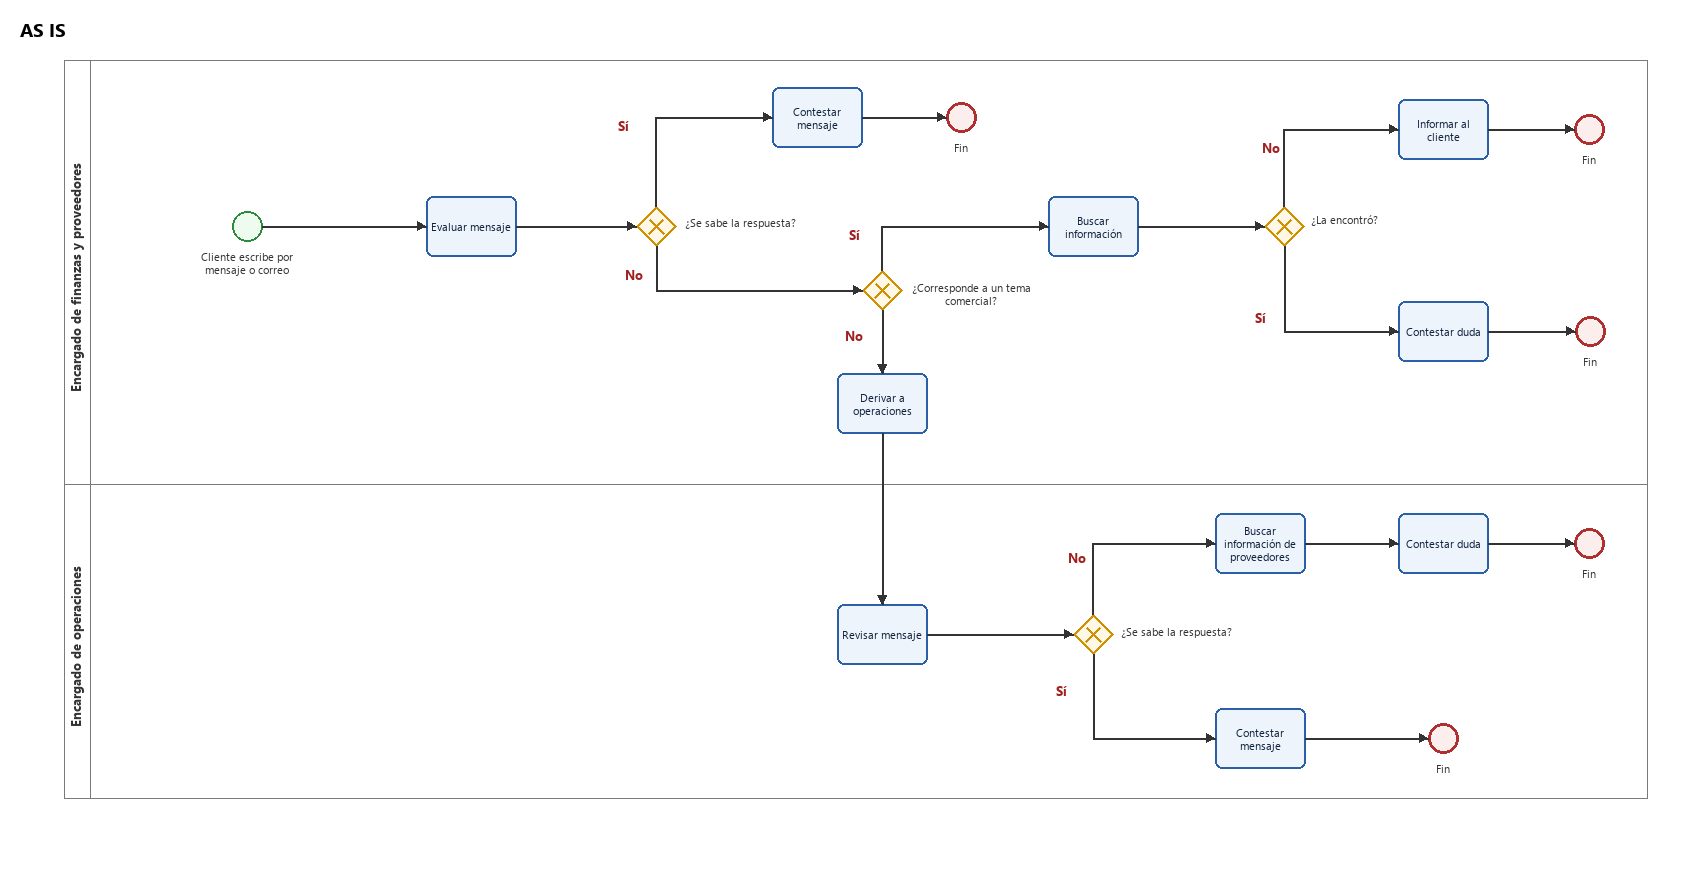
\includegraphics[width=\linewidth,height=0.84\textheight,keepaspectratio]{atencion-ASIS.png}
\caption{Atención de consultas de clientes --- AS-IS (Entrega~1).\label{fig:aten_asis}}
\end{figure}
\end{landscape}

\begin{landscape}
\thispagestyle{plain}
\begin{figure}[H]
\centering
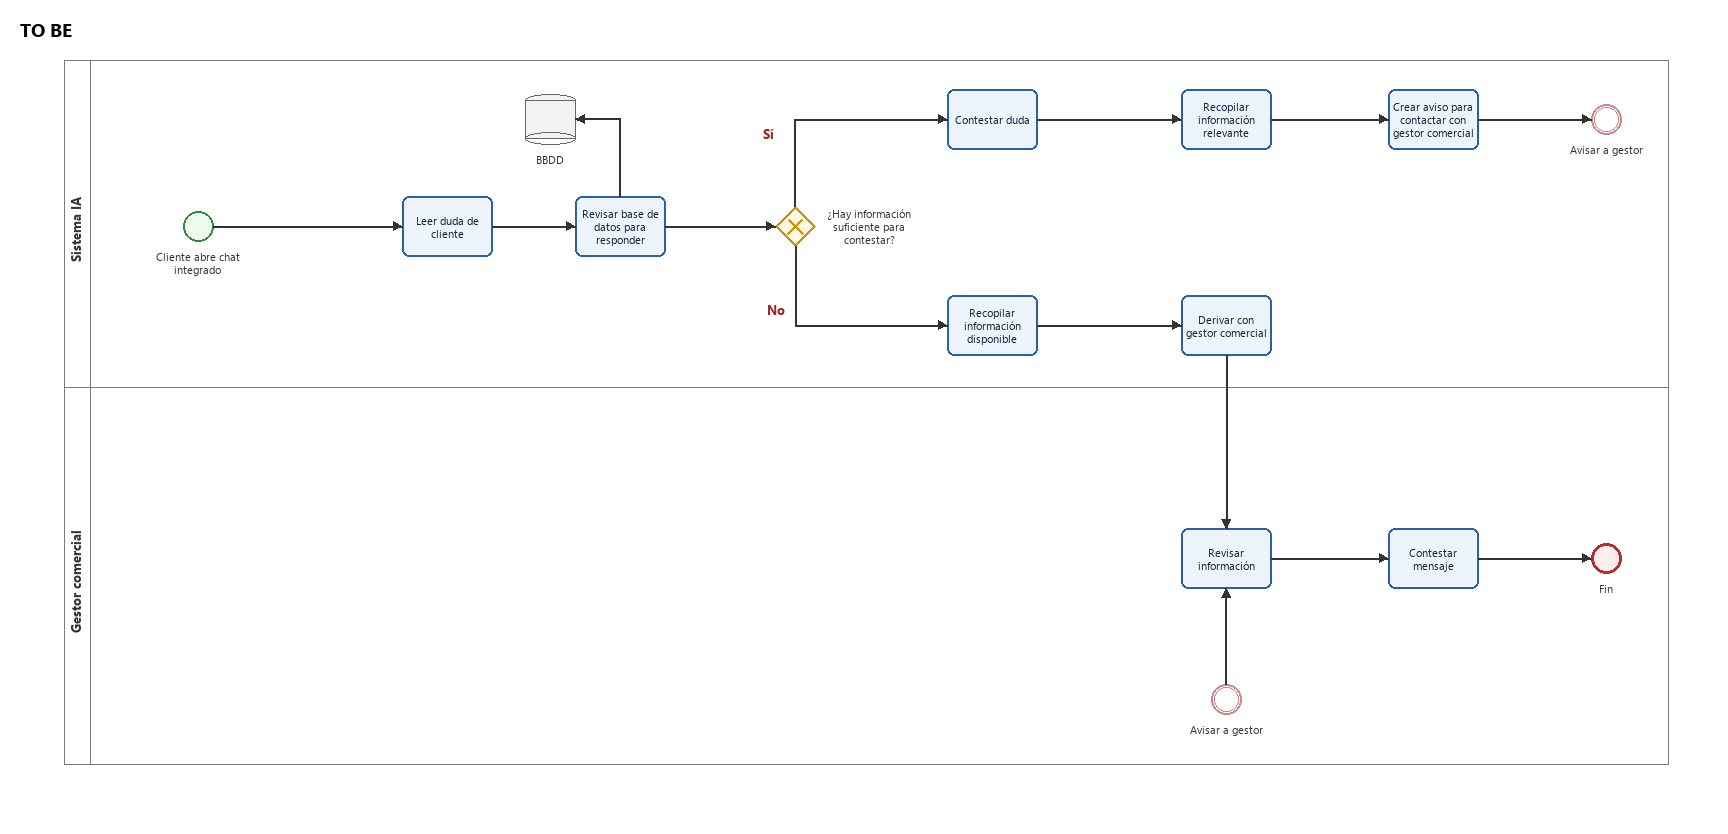
\includegraphics[width=\linewidth,height=0.84\textheight,keepaspectratio]{atencion-TOBE.png}
\caption{Atención de consultas de clientes --- TO-BE con asistente y derivación (continuidad en BD 3FN).\label{fig:aten_tobe}}
\end{figure}
\end{landscape}

\begin{landscape}
\thispagestyle{plain}
\begin{figure}[H]
\centering
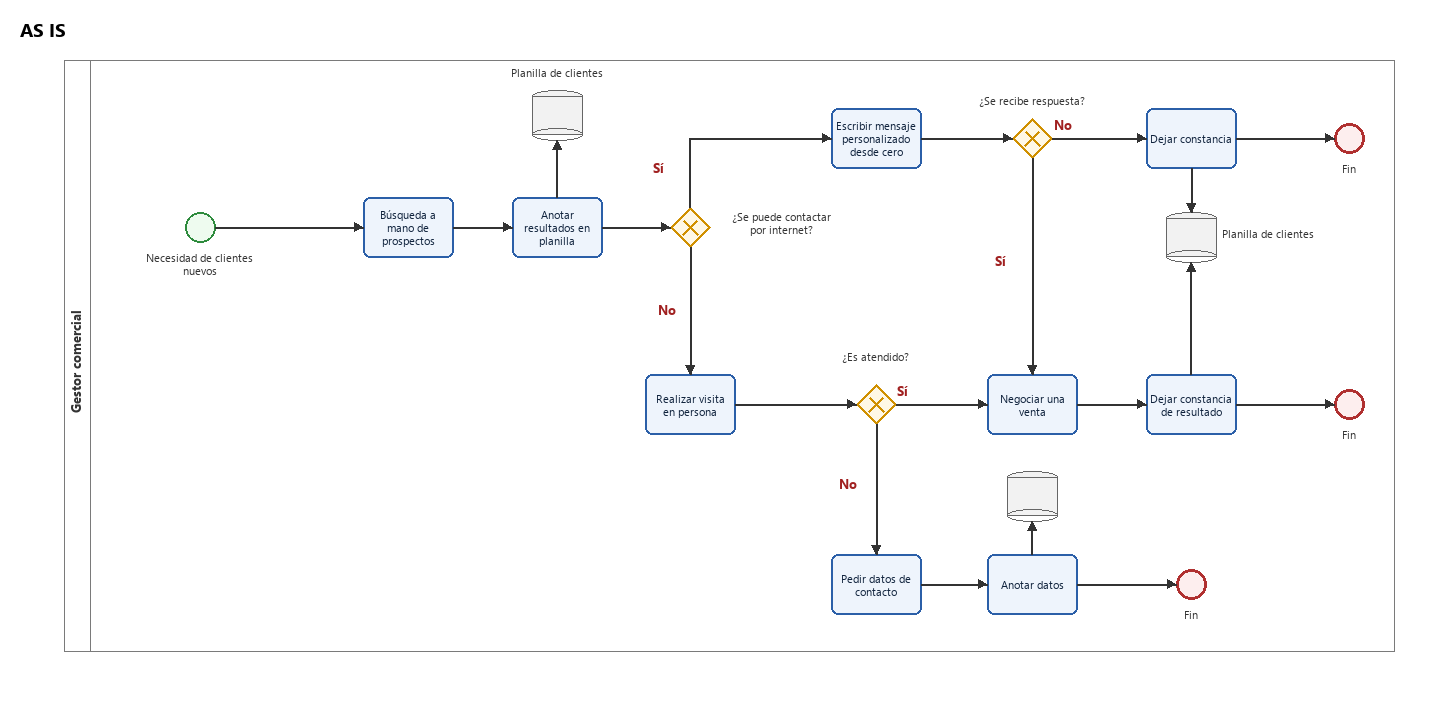
\includegraphics[width=\linewidth,height=0.84\textheight,keepaspectratio]{busqueda-ASIS.png}
\caption{Línea base AS-IS de búsqueda y prospección manual de clientes (Entrega~1).\label{fig:busq_asis}}
\end{figure}
\end{landscape}

\begin{landscape}
\thispagestyle{plain}
\begin{figure}[H]
\centering
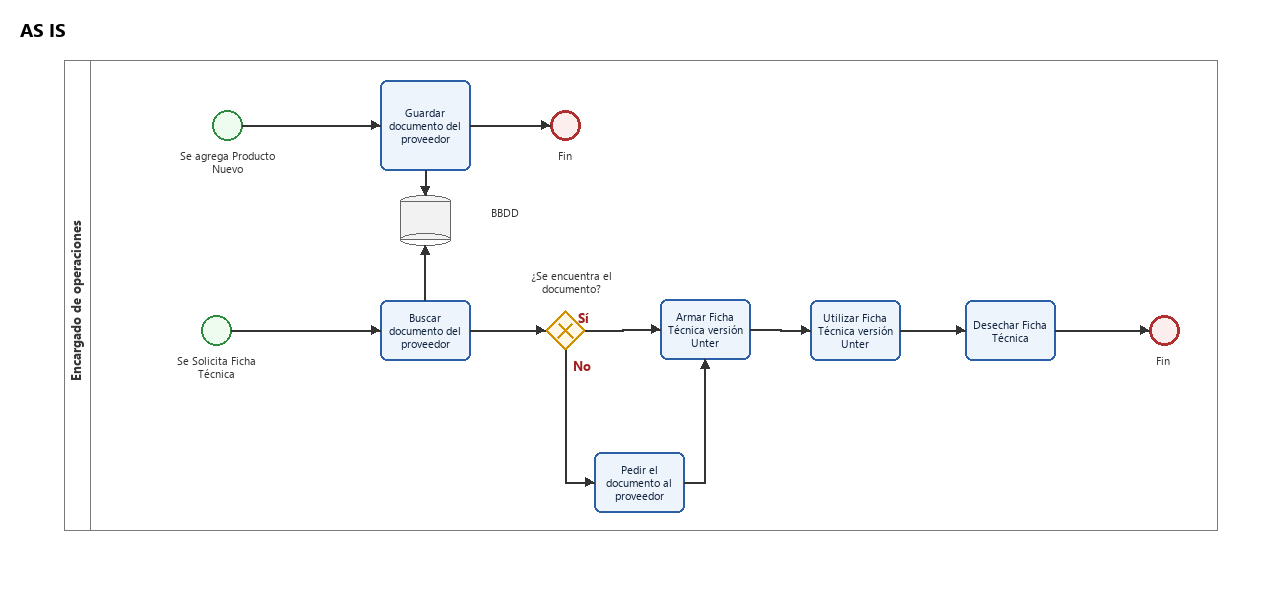
\includegraphics[width=\linewidth,height=0.84\textheight,keepaspectratio]{fichas-ASIS.png}
\caption{Línea base AS-IS de armado manual de fichas técnicas (Entrega~1).\label{fig:fich_asis}}
\end{figure}
\end{landscape}

\end{document}
